
\documentclass[twocolumn]{aastex62}


\newcommand{\vdag}{(v)^\dagger}
\newcommand\aastex{AAS\TeX}
\newcommand\latex{La\TeX}

%% Reintroduced the \received and \accepted commands from AASTeX v5.2
%\received{July 1, 2016}
%\revised{September 27, 2016}
%\accepted{\today}
%% Command to document which AAS Journal the manuscript was submitted to.
%% Adds "Submitted to " the arguement.
%\submitjournal{ApJ}


\shorttitle{\aastex\ G240}
\shortauthors{Liu et al.}


\begin{document}

\title{THE ISOTHERMAL OUTFLOW IN THE MASSIVE STAR-FORMING REGION G240.31+0.07}

\correspondingauthor{Keping Qiu}
\email{kpqiu@nju.edu.cn}

\author[0000-0002-4774-2998]{Junhao Liu}
\affil{School of Astronomy and Space Science, Nanjing University, 163 Xianlin Avenue, Nanjing 210023, P.R.China}

\author{Keping Qiu}
\affil{School of Astronomy and Space Science, Nanjing University, 163 Xianlin Avenue, Nanjing 210023, P.R.China}
\affiliation{Key Laboratory of Modern Astronomy and Astrophysics (Nanjing University), Ministry of Education, Nanjing 210023, P.R.China}

\author{Friedrich Wyrowski}
\affiliation{Max-Planck-Institut f{\"u}r Radioastronomie, Auf dem H{\"u}gel 69, 53121 Bonn, Germany}

\author{Karl Menten}
\affiliation{Max-Planck-Institut f{\"u}r Radioastronomie, Auf dem H{\"u}gel 69, 53121 Bonn, Germany}

\author{Rolf G{\"u}sten}
\affiliation{Max-Planck-Institut f{\"u}r Radioastronomie, Auf dem H{\"u}gel 69, 53121 Bonn, Germany}

\author[0000-0002-6368-7570]{Yue Cao}
\affil{School of Astronomy and Space Science, Nanjing University, 163 Xianlin Avenue, Nanjing 210023, P.R.China}

\author{Yuwei Wang}
\affil{School of Astronomy and Space Science, Nanjing University, 163 Xianlin Avenue, Nanjing 210023, P.R.China}

\begin{abstract}
%We present Atacama Pathfinder Experiment (APEX) observations toward the massive star-forming region \objectname{G240.31+0.07} in the CO (3-2), (6-5), and (7-6) lines. These lines have traced the previously detected bipolar outflow and show similarity in morphology. The CO (3-2), (6-5), and (7-6) data were complemented with previously observed CO (2-1) data. All line ratios of the four transitions are remarkably constant with velocity. Using the CO (3-2), (6-5), and (7-6) data and the complementary CO (2-1) data, we estimate the physical parameters of the outflow as functions of the gas velocity, by the means of the rotalation diagram analysis and the large velocity gradient (LVG) analysis. Our analysing results reveal that the the outflow is isothermal and has a temperature of $\sim$ 50 K. This value is warmer than previously adopted $\sim$ 30 K. We also find a decreasing trend of CO column density with gas velocity. In addition, the modeling results reveal that the outflowing gas is thermalized and has gas densities of $ > 10^5$ cm$^{-3}$. A decreasing trend of gas density with velocity is detected if assumptions of a constant CO abundance ratio and a constant velocity gradient are valid. The isothermal state and the decreasing density-velocity trend are qualitatively consistent with the wide-angle wind-driven model. Since wide-angle winds associated with low-mass YSOs are related to disk-accretion process, the wide-angle wind-driven G240 outflow provides evidence that high-mass stars up to late-O types can form via disk-mediated accretion.
We present Atacama Pathfinder Experiment (APEX) observations toward the massive star-forming region \objectname{G240.31+0.07} in the CO J = 3-2, 6-5, and 7-6 lines. We detect a parsec-sized, bipolar, and high velocity outflow in all the lines, which allow us, in combination with the existing CO J = 2-1 data, to perform a multi-line analysis of physical conditions of the outflowing gas. The CO 7-6/6-5, 6-5/3-2, and 6-5/2-1 ratios are found to be nearly constant over a velocity range of $\sim 5-25$ km s$^{-1}$ for both blueshifted and redshifted lobes. We carry out rotation diagram and large velocity gradient (LVG) calculations of the four lines, and find that the outflow is approximately isothermal with a gas temperature of ∼ 50 K, and that the the CO column density clearly decreases with the outflow velocity. If the CO abundance and the velocity gradient do not vary much, the decreasing CO column density indicates a decline in the outflow gas density with velocity. By comparing with theoretical models of outflow driving mechanisms, our observations and calculations suggest that the massive outflow in G240.31+0.07 is being driven by a wide-angle wind and further support a disk mediated accretion at play for the formation of the central high-mass star.
\end{abstract}

\keywords{ISM:  individual objects (\objectname{G240.31+0.07}) - ISM: jets and outflows - stars: formation}

\section{Introduction}
Bipolar molecular outflows, mostly observed via CO, HCO$^+$ and their isotopes, are a common phenomenon associated with young stellar objects (YSOs) of all masses \citep{2001ApJ...552L.167Z, 2002A&A...383..892B, 2004A&A...426..503W, 2005AJ....129..330W,  2015MNRAS.453..645M}. It is believed that molecular outflows trace the accretion-powered ejections in sites of low-mass star formation. As molecular outflows impact the surrounding material and the parent cloud significantly, they play an important role in the star formation process. Though molecular outflows have been well studied, the driving mechanism of molecular outflows remains unknown. Molecular outflows from low-mass protostars were thought to be entrained by wide-angle winds \citep{1991ApJ...370L..31S, 2001ApJ...557..429L}, or by jet bow shocks \citep{ 1993A&A...278..267R, 1993ApJ...414..230M, 2001ApJ...557..429L}. Though the wind-driven model and the jet-driven model can each explain the characteristics of some observed outflows, none of them are capable of producing the observed features of all types of outflows \citep{2000ApJ...542..925L, 2002ApJ...576..294L}. In order to explain different features of various types of outflows associated with low-mass YSOs simultaneously, two-component models with both highly collimated jet and wide-angle wind have been developed \citep{2000prpl.conf..789S, 2006ApJ...641..949B, 2006MNRAS.365.1131P, 2006ApJ...649..845S, 2007prpl.conf..277P, 2008ApJ...676.1088M}.

Massive molecular outflows are more problematic than their low-mass counterparts. Though observations have shown that the morphology and kinematics of some outflows driven by massive YSOs are very similar to the outflows driven by low mass YSOs \citep[][]{1998ApJ...507..861S, 2002A&A...387..931B, 2009ApJ...696...66Q, 2011MNRAS.415L..49R}, there is a lack of detection of extremely collimated outflows and circumstellar disks towards sources more massive than early B-type YSOs \citep{2007prpl.conf..245A}. Thus, it is not clear whether massive stars form as a scaled-up version of low-mass stars or they form in a different way. Due to the rarity and typically large distances of high-mass YSOs, the sample of individual studies towards outflows driven by massive YSOs is still small. And there is little theoretical work on modeling outflows from high-mass YSOs. Many questions, e.g., how the outflows from massive YSOs are accelerated, how they differ from low-mass outflows, and how they affect the high-mass star-forming processes, are still unanswered. It is essential to address these questions by studying more outflows associated with high-mass star-forming regions. 

Most previous studies of outflows have used low-J rotational transitions of CO (transitions up to J$_u$ = 3, with upper-state energies E$_u$ up to 30 K), which are easily excited at low temperatures, to characterize the relatively cold and extended molecular gas in morphology and kinematics. These low-J CO emission lines can be easily observed from the ground-based facilities. Due to atmospheric limits, mid-J CO lines (referring to CO (6-5) and CO (7-6) throughout this paper, with  E$_u$ up to 150 K), which are less affected by ambient gas, are not commonly observed. In several studies, mid-J CO transitions have been reported to trace the warm gas (T $>$ 50 K) in outflows of low-mass and intermediate-mass YSOs \citep{2009A&A...501..633V, 2009A&A...507.1425V, 2012A&A...542A..86Y, 2016A&A...587A..17V}.  By comparing multi-line CO observations (both low-J and mid-J) with the results of non-LTE radiative transfer models, the physical properties (temperature, gas density and CO column density) of the outflowing gas could be well constrained \citep{2015A&A...581A...4L}. 

This paper is a follow-up study of the \objectname{G240.31+0.07} (hereafter \objectname{G240}) outflow \citep{2009ApJ...696...66Q}. We report the 12-m submillimeter Atacama Pathfinder Experiment Telescope\footnote{    The Atacama Pathfinder Experiment Telescope is a collaboration between the Max-Planck-Institut f$\ddot{\mathrm{u}}$r Radioastronomie, the European Southern Observatory, and the Onsala Space Observatory.} (APEX) observations of \objectname{G240}, an active high-mass star-forming region which is associated with the YSO \objectname{IRAS 07427-2400} and located at a distance of 5.41 kpc \citep{2015PASJ...67...69S}. It harbors an ultracompact HII region and is associated with OH and H$_2$O masers \citep{1993AJ....105.1495H, 1997MNRAS.289..203C, 1998AJ....116.1897M, 1999ApJS..123..487M, 2003MNRAS.341..551C}. Its far-infrared luminosity of 10$^{4.7}$ L$_\sun$ is consistent with a spectral type O8.5 zero-age main-sequence star \citep{1998AJ....116.1897M}. \citet{2009ApJ...696...66Q} presented a high resolution interferometric study at 1.3 mm and resolved the central part of \objectname{G240} into three dusty cores MM1, MM2, and MM3. \citet{2003A&A...412..175K} mapped the CO (3-2) emission with a 20${\arcsec}$ beam and found a prominent bipolar outflow at a position angle (PA) of 132${\degr}$ and a weaker component at PA $\sim$ 101${\degr}$. With C$^{18}$O (2-1) observations, \citet{2003A&A...412..175K} found the cloud velocity ($v_{\mathrm{cloud}}$) with respect to the local standard of rest to be $\sim$ 67.5 km s$^{-1}$. Recently, \citet{2009ApJ...696...66Q} presented a detailed single dish and interferometric study of $^{12}$CO (2-1) and $^{13}$CO (2-1) emissions and detected a bipolar, wide-angle, quasi-parabolic molecular outflow. In addition, \citet{2014ApJ...794L..18Q} reported the detection of an hourglass magnetic field aligned within 20${\degr}$ of the outflow axis.

In this paper, we present a CO multi-transition (2-1, 3-2, 6-5, 7-6) study towards the \objectname{G240} outflow. With rotation diagram (RD) analysis and large velocity gradient (LVG) calculations, we estimate the physical parameters of the outflow as functions of gas velocity. We then discuss the results of the analyses.



\section{OBSERVATIONS}

The APEX observations were conducted on . CO (6-5) and CO (7-6) were observed simultaneously. The pointing error of CO (6-5) and (7-6) was fixed by comparing them with the CO (2-1) data.
\section{Results}
\subsection{CO emission maps}

\begin{figure*}[htbp]
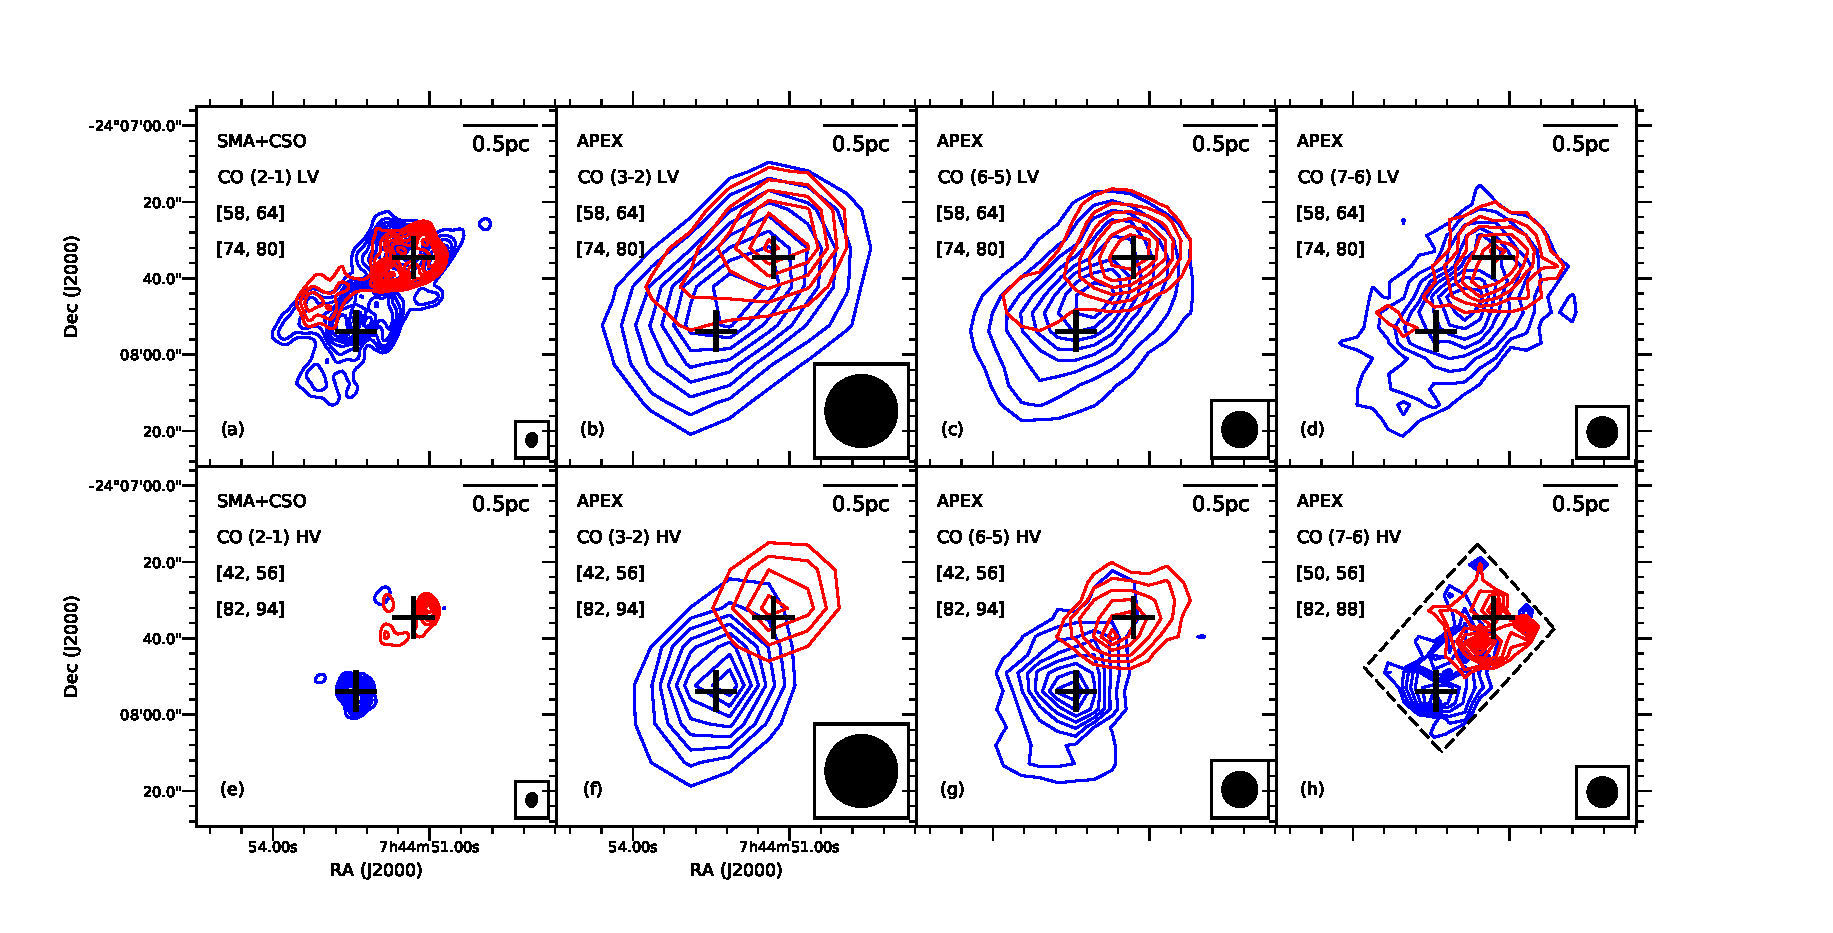
\includegraphics[scale=.65]{./fig/ori_contourall.eps}
\caption{(a)-(d) Low-velocity CO J = 2-1, 3-2, 6-5, 7-6 emissions, integrated from 58 to 64 km s$^{-1} $ for the blueshifted lobe (blue) and from 74 to 80 km s$^{-1}$ for the redshifted lobe (red); (e)-(f) High-velocity CO J = 2-1, 3-2 emissions,  integrated from 42 to 56 km s$^{-1} $ for the blueshifted lobe (blue) and from 82 to 94 km s$^{-1}$ for the redshifted lobe (red); (g) High-velocity CO J = 6-5 emission, integrated from 44 to 56 km s$^{-1} $ for the blueshifted lobe (blue) and from 82 to 92 km s$^{-1}$ for the redshifted lobe (red) (h) High-velocity CO J = 7-6 emission, integrated from 46 to 56 km s$^{-1} $ for the blueshifted lobe (blue) and from 82 to 90 km s$^{-1}$ for the redshifted lobe (red). For (a)-(g), the contour levels start from 20\% and continue at steps of 10\% of the peak emission. For (h), the contour levels start from 30\% and continue at steps of 10\% of the peak emission. Edge channels are masked out because of high noise levels. The black star marks the position of a H$_2$O maser spot which is associated with IRAS 07427-2400 \citep{2015PASJ...67...69S}. The beam of each observational dataset is shown in the lower right corner of each panel. \label{fig:figcontour}}
\end{figure*}

The CO 3-2, 6-5 and 7-6 emissions are detected (with obvious outflow signatures and with peak intensities $>$ 2 $\sigma_{rms}$) in velocity ranges from 42 km s$^{-1}$ to 94 km s$^{-1}$, 44 km s$^{-1}$ to 92 km s$^{-1}$, and 46 km s$^{-1}$ to 90 km s$^{-1}$, respectively. Figure \ref{fig:figcontour} shows the integrated low-velocity (LV) and high-velocity (HV) emissions of the four lines. The velocity ranges chosen to highlight the LV and HV components of the outflowing gas follow those in \citet{2009ApJ...696...66Q}, except that the channels with no detections were excluded for the HV component. The morphologies of the bipolar outflow seen in the emission from the CO 3-2, 6-5 and 7-6 lines are very similar. Due to the coarser angular resolution, the wide-angle structure seen in the higher resolution CO 2-1 image is not seen in the CO 3-2, 6-5, 7-6 maps.

\subsection{Physical conditions of the outflow}
\subsubsection{Methodology}

\begin{figure}[tbp]
\plotone{./fig/ratio.eps}
\caption{Ratios of the main-beam brightness temperatures of different CO lines at different velocities. Blue symbols denote the measurements from the blueshifted lobe, and red symbols the redshifted lobe. The $V_{\mathrm{outflow}}$ shown here is related to the cloud velocity $v_{\mathrm{cloud}}$ by the relation: $V_{\mathrm{outflow}}$ = $\mid$ $v_{\mathrm{outflow}}$ - $v_{\mathrm{cloud}}\mid$, where $v_{\mathrm{outflow}}$ is the outflow velocity with respect to the local standard of rest. \label{fig:figratio}}
\end{figure}

The physical conditions of the outflow can be constrained by comparing the observed line intensities with the results of statistical-equilibrium calculations. To study the four lines at the same spatial resolution, the CO 2-1, 6-5 and 7-6 maps were reconstructed with the same beam of the CO 3-2 map. The average rms noise levels are $\sim$0.004 K, $\sim$0.04 K and $\sim$0.1 K for the convolved CO 2-1, 6-5 and 7-6 data, respectively. For both lobes of the outflow, the CO line intensities were measured at roughly the peak positions of the HV components of the convolved CO maps (marked as two crosses in every panel of Figure \ref{fig:figcontour}), and were then used in the following analysis. Figure \ref{fig:figratio} shows the ratios of the main-beam brightness temperatures ($T_{\mathrm{mb}}$) of different CO lines as functions of velocity. The CO 7-6/6-5, 6-5/3-2, and 6-5/2-1 ratios are remarkably constant over a velocity range of $\sim 5-25$ km s$^{-1}$ with respect to the cloud velocity. In the analysis, we only used channels of $\le$ 60 km s$^{-1}$ and $\ge$ 74 km s$^{-1}$ to avoid contaminations from the ambient gas, and we excluded channels of $<$ 46 km s$^{-1}$ or $>$ 90 km s$^{-1}$ because of their low signal-to-noise ratios. The outflow emission was analyzed in each 2 km s$^{-1}$ bin. Considering that the $^{13}$CO 2-1 emission was only marginally detected in the outflowing gas with high sensitivity observations \citep{2009ApJ...696...66Q}, we assumed the four $^{12}$CO lines to be optically thin. In the optically thin case, the source size is degenerate with column density (see section \ref{section:density}). We didn't correct the observed line intensities for beam filling factors, so the derived CO column densities should be considered as beam-averaged values. In the calculation, errors on line intensities took into account both the calibration error and the rms noise. 
%(R.A., decl.)$_{J2000}$ = ($07^h44^m52^s.4, -24^d7^m53^s.8$) and (R.A., decl.)$_{J2000}$ = ($07^h44^m51^s.3, -24^d7^m34^s.6$)
%We note that the offsets of the peak positions are within $\sim$ 3$\arcsec$ for different lines at different velocities.
%The uncertainty of the observed intensity mainly consists of two parts: the calibration error and the rms noise. At low velocities, the calibration uncertainty dominates the intensity uncertainty, whereas the rms noise is dominant at high velocities. A combination of the rms noise and the calibration error $\sigma_{obs} = (\sigma_{cal}^2 + \sigma_{rms}^2)^{\frac{1}{2}}$ was used as the observational uncertainty in the belowing analyses.
%errors take into account both the rms noise and the calibration uncertainties.

\subsubsection{Rotation diagram analysis\label{subsec:RD}}

\begin{figure}[tbp]
\plotone{./fig/RD.eps}
\caption{A rotation diagram for CO at 84 km s$^{-1}$. The fitted line shows the Boltzmann distribution of the rotational populations. The line represents a rotational temperature of 48.5 K and a total column density of 2.0 $\times$ 10$^{15}$ cm$^{-2}$. The black solid circles show the data with error bars. \label{fig:figrd}}
\end{figure}

Firstly, we performed a simple rotation diagram (RD) analysis \citep{1999ApJ...517..209G} to estimate the excitation conditions of the outflowing gas under the assumption of local thermal equilibrium (LTE). The population of each energy level is given by 
\begin{equation}
N_{\mathrm{up}} = \frac{N_\mathrm{CO}}{Z} g_\mathrm{up} e^{-E_\mathrm{up}/kT_\mathrm{kin}},
\end{equation}
where $N_\mathrm{up}$ is the column density in the upper state, $g_\mathrm{up}$ the statistical weight of the upper state, $E_\mathrm{up}$ the upper energy level, $k$ the Boltzmann constant, and $Z$ is the partition function. The rotation diagram for CO at 84 km s$^{-1}$ is shown in Figure \ref{fig:figrd} as an example. The different energy levels are well reproduced by a single-component, indicating that the four transitions are probing the same volume of gas. Similar rotation diagram patterns with one gas component are found at other velocities. The derived gas temperature and CO column density as functions of the gas velocity are shown in Figure \ref{fig:figrelation}.

\subsubsection{Large velocity gradient analysis\label{subsec:LVG}}

\begin{figure*}[!tbp]
\gridline{\fig{./fig/chiimage_nco_paper.eps}{0.5\textwidth}{(a)}
        \fig{./fig/chiimage_nh2_paper.eps}{0.5\textwidth}{(b)}}
 \gridline{\fig{./fig/chiimage_tkin_paper.eps}{0.5\textwidth}{(c)}
      }
\caption{(a)-(c) The $\chi^2$ distribution at 84 km s$^{-1}$ in the [$T$, $n$], [$T$, $N$] and [$n$, $N$] planes, with the third parameter fixed to the value of the best fitting result at this velocity. The lower limit of gas density is 1.8 $\times$ 10$^{5}$ cm$^{-3}$. The best-fit solution is obtained for $T$ =  46.1 K and N = 2.2 $\times$ 10$^{15}$ cm$^{-2}$. The $\chi^2_{\mathrm{red}}$ of the best-fit solution is 1.00. The Solid white contours show the 1$\sigma$ confidence levels. \label{fig:figchi}}
\end{figure*}

Secondly, the non-LTE radiative transfer code RADEX \citep{2007A&A...468..627V} was used to better constrain the gas density ($n$), the kinetic temperature ($T$) and the CO column density ($N$) of the outflowing gas. RADEX employs the the LVG approximation. We built a large grid of LVG models varying the three parameters ($n$, $T$ and $N$), and obtained the best fitting results by minimizing the $\chi^2$ calculated from the observed intensities and the model intensities. With four lines observed and three parameters to constrain, our fitting had one degree of freedom. In Figure \ref{fig:figchi}, the fitting results at 84 km s$^{-1}$ are shown as examples of the distributions of $\chi^2$. Only one minimum of $\chi^2$ is found in the [$T$, $N$] plane. In the [$T$, $n$] and [$n$, $N$] planes, the $\chi^2$ distributions show that the gas is thermalized and no upper limits to the H$_2$ density could be derived, which confirms the LTE assumption of the rotation diagram analysis. Similar $\chi^2$ distribution patterns were found at other velocities. The best-fit solutions at different velocities are very close to the results of the rotation diagram (see Figure \ref{fig:figrelation}). The reduced $\chi^2$ ($\chi^2_{\mathrm{red}}$) of the best fitting results varies from 0.10 to 1.72 at different velocities. We derive the uncertainties of each parameter from the 1$\sigma$ confidence region in the 3D parameter space at the velocities where $\chi^2_{\mathrm{red}} \sim 1$ as the representative parameter uncertainties. The uncertainty of CO column densities is $\sim$ 10 \%. The 1$\sigma$ confidence range of the temperature is about 40 K - 60 K. And the gas density is $>$ 10$^5$ cm$^{-3}$ over the entire outflow. The modeling results also predict that the four transitions are optically thin in the outflowing gas, which is consistent with our assumptions. Figure \ref{fig:figsed} shows the comparison of the observed CO intensities with the LVG modeling results in each velocity bin. 
% Though the best-fitted $\chi^2_{\mathrm{red}}$ varies, the $\chi^2_{\mathrm{red}}$ distribution profiles show similarity in morphology at different velocities, indicating that the uncertainties of the fitted parameters may have similar levels at different velocities.

\subsubsection{$T$-$V$ and $N$-$V$ relations}

\begin{figure*}[!tbp]
\gridline{\fig{./fig/tv_paper.eps}{0.5\textwidth}{(a)}
          \fig{./fig/Nv_paper.eps}{0.5\textwidth}{(b)}
          }
\caption{$T$-$V$ and $N$-$V$ diagrams of the G240 outflow, estimated from the rotation diagram analysis (blue ``x'' markers for the blue lobe and red ``x'' markers for the red lobe) and the LVG analysis (blue open squares for the blue lobe and red open squares for the red lobe). \label{fig:figrelation}}
\end{figure*}

In Figure \ref{fig:figrelation}, the $T$-$V$ diagram shows that the gas is approximately isothermal with a gas temperature of $\sim$ 50 K, while the $N$-$V$ diagram shows that the CO column density in each 2 km s$^{-1}$ bin decreases from $\sim 2 \times 10^{16} $ cm$^{-2}$ at $\sim \pm$ 7 km s$^{-1}$ down to $\sim 4 \times 10^{14}$ cm$^{-2}$ at $\sim \pm$ 22 km s$^{-1}$. We compared the model intensities with line intensities measured at several different positions, and found that the modeling results are similar to those represented in Figure \ref{fig:figrelation}. Thus, a systematic bias of position offsets was excluded.
%Thus, we exclude the systematic bias from choices of positions for measuring the line intensities.





\section{DISCUSSION}\label{discussion}

Though the morphology and kinematics of molecular outflows have been widely studied, there is a lack of studies towards some other physical properties (e.g., the variation of temperature and density with velocity). CO mid-J observations as complements of existed low-J observations are required to constrain the temperature and density of the molecular outflows as a function of velocity, while these mid-J observations are challenging because of atmospheric limits. There are only several studies on the the $T-V$ relation of molecular outflows. A rising CO 3-2/6-5 ratio is observed towards the outflow associated with low-mass YSO HH 46 IRS 1\citep{2009A&A...501..633V}. With the density assumed to be constant, the rising ratios at more extreme velocities correspond to lower kinetic temperatures. In the case of the outflow associated with low-mass protostars NGC 1333 IRAS 4A and  IRAS 4B, the CO 3-2/6-5 ratios are remarkably constant with velocity \citep{2012A&A...542A..86Y}. With the assumption of constant density, the constant ratios indicate constant temperatures. \citet{2012ApJ...744L..26S} have imaged the extremely high velocity (EHV) outflow in CO (2-1) and CO (3-2) associated with the high-mass YSO G5.89-0.39. With the assumption of a canonical CO fractional abundance of 10$^{-4}$, an increasing trend of temperature with outflow velocity is found by performing a LVG analysis. Using the CO (6-5), (7-6) and (16-15) lines, \citet{2015A&A...584A..70L} performed a RD analysis towards the G5.89-0.39 outflow and found a decreasing trend of temperature with increasing velocities. This disagreement seen in results of \citet{2012ApJ...744L..26S} and \citet{2015A&A...584A..70L} could be due to different angular resolutions (3${\arcsec}$.4 compared to 14${\arcsec}$.5 ) and different energy range ($\Delta E_u \sim 17 $K compared to $\Delta E_u \sim 600 $K). The different $T-V$ relations found in different outflows and in different angular scales reveal the complexity of molecular outflows. However, with only two or three lines observed, their derived $T-V$ relations must be deduced from fixing other physical parameters, e.g., constant density or constant canonical CO fractional abundance, or from the assumption that the different transitions can be discribed with the same excitation temperature (LTE). To get more proper estimations of the pysical parameters of the molecular outflow, multi-line studies of CO and more sophisticated methods (e.g. LVG) are required.

The LVG analysis and the RD analysis reveal that the G240 outflow is isothermal and has a temperature of $\sim$ 50 K . This value is consistent with temperatures in excess of 50 K probed by \citet{2016A&A...587A..17V} for outflows associated with intermediate-mass protostars, and slightly lower than temperatures of outflows associated with low-mass protostars \citep{2009A&A...501..633V, 2012A&A...542A..86Y}. The isothermal state rules out the jet-driven bow shock models, which predicts temperature rising with outflow velocity and distance, and provides evidence for the wind-driven model \citep{2007prpl.conf..245A}. As molecular cooling dominates the cooling of the shocked material in the outflow at temperatures below 10$^4$ K \citep{1997IAUS..182..181H} and the cooling rate increases as $n^2$, molecular cooling is very efficient for the typical density of a wind-driven outflow. Thus, an isothermal state could be reached in a wind-driven outflow. We noticed that there are faint bow-shaped H$_{2}$ features near the YSO \objectname{IRAS 07427-2400}, suggesting that the jet-driven outflows may also exist. However, as the average T-V relation of the outflowing gas agrees with the wind-driven model and the kinematics and morphology of the molecular outflow can also be qualitatively interpreted by the wide-angle wind-driven model \citep{2009ApJ...696...66Q}, we conclude that even if the jet-driven outflows and the wind-driven outflows were coexisting in the G240 outflow, the wide-angle wind entrainment plays a more important role in driving the G240 outflow. It should be noted that, most existing outflow models have parameters typical of outflows driven by low-mass YSOs. It is necessary to compare the observational results of outflows driven by high-mass YSOs with models of similar physical conditions. Statics of outflows associated with high-mass star-forming regions are also essential for us to better understand the driven mechanism of massive outflows and the forming process of high-mass stars.

The LVG analysis reveals that the lower limits of gas densities are $\sim 10^5$ cm$^{-3}$ at the velocities where $\chi^2_{\mathrm{red}} \sim 1$. We have found a decreasing trend of the beam averaged CO column density with gas velocity. As shown in the $N$-$V$ diagram of Figure \ref{fig:fig4}, for each velocity bin (2 km s$^{-1}$), the beam averaged CO column density drops from $\sim 2 \times  10^{16} $ cm$^{-2}$ to $\sim 8 \times 10^{14}$ cm$^{-2}$ within 15 km s$^{-1}$. In the optically thin case, the beam averaged CO column density could be related to gas density $n_{\mathrm{H}_2}$ through the expression: 
\begin{equation}
N_{\mathrm{CO}} = n_{\mathrm{H}_2} \times \Delta V \times \frac{1}{dv/dr} \times X_{\mathrm{CO}} \times f_{\mathrm{b}}, 
\end{equation}
where $f_{\mathrm{b}}$ is the beam filling factor, $X_{\mathrm{CO}}$ the CO/H$_2$ abundance ratio, $\Delta V$ the velocity interval and $dv/dr$ is the velocity gradient. A drop in $N_{\mathrm{CO}}$ at more extreme velocities indicates the decrease of one or serveral of these parameters. 
To explore how the effect of beam dilution influence our results, we vary the beam filling factors from 0.2 to 1 and then perform the LVG analysis again. We find that modelling with different beam filling factors mainly affect the $N$-$V$ diagram, with minor change in the $T$-$V$ diagram and density limits. This could be resulted from the degeneracies of the beam filling factor with CO column density in the optically thin case. 

As shown in Figure 3 of \citet{2009ApJ...696...66Q}, the source size are $\sim 20\arcsec$ and $\sim 10\arcsec$ at the velocities of $\sim \pm$ 6 km s$^{-1}$ and $\sim \pm$ 20 km s$^{-1}$ with respect to the cloud velocity, corresponding to beam filling factors of $\sim$ 0.5 and $\sim$ 0.2, respectively. Considering the 2.5 times drop in the beam filling factor, the 25 times drop in the beam averaged CO column density indicates $\sim$ 10 times decrease in the CO column density. Due to the lack of other informations, we cannot assess whether the CO abundance ratio or the velocity gradient has attributed to the drop of CO column density at high velocities. As shown in \citet{2007prpl.conf..245A}, the wind-driven models predict that the wind density decreases with velocity and distance from the driving source. Thus, if we assume the CO abundance ratio and the velocity gradient to be constant, the decrease of CO column density could be interpreted by a decrease of gas density with velocity.
\section{SUMMARY}\label{summary}

We have presented a CO multi-transition (CO 2-1, 3-2, 6-5, 7-6) study towards the molecular outflow of the high-mass star-forming region \objectname{G240}. The morphologies seen in four lines are very similar. With the LVG analysis, we have constrained the temperatures to $\sim$ 50 K and found a decreasing trend of CO column density with gas velocity. We also constrain the H$_2$ density to values higher than $n \sim 10^5$ cm$^{-3}$ and found that the outflowing gas is thermalized. With the RD analysis, we found similar results in the temperature and the CO column density. The T-V relation of the G240 outflow agrees well with the wide-angle wind-driven model. Assuming a constant CO abundance
ratio and a constant velocity gradient, we detect a decreasing gas density with velocity, which is also consistent with the wide-angle wind-driven model. 

%\acknowledgments
%We thank

\begin{thebibliography}{}
\bibitem[Arce et al.(2007)]{2007prpl.conf..245A} Arce, H.~G., Shepherd, D., Gueth, F., et al.\ 2007, Protostars and Planets V, 245 
\bibitem[Banerjee \& Pudritz(2006)]{2006ApJ...641..949B} Banerjee, R., \& Pudritz, R.~E.\ 2006, \apj, 641, 949 
\bibitem[Beuther et al.(2002a)]{2002A&A...383..892B} Beuther, H., Schilke, P., Sridharan, T.~K., et al.\ 2002, \aap, 383, 892
\bibitem[Beuther et al.(2002b)]{2002A&A...387..931B} Beuther, H., Schilke, P., Gueth, F., et al.\ 2002, \aap, 387, 931 
\bibitem[Caswell(1997)]{1997MNRAS.289..203C} Caswell, J.~L.\ 1997, \mnras, 289, 203 
\bibitem[Caswell(2003)]{2003MNRAS.341..551C} Caswell, J.~L.\ 2003, \mnras, 341, 551 
\bibitem[Choi et al.(2014)]{2014ApJ...790...99C} Choi, Y.~K., Hachisuka, K., Reid, M.~J., et al.\ 2014, \apj, 790, 99 
\bibitem[Frank et al.(2014)]{2014prpl.conf..451F} Frank, A., Ray, T.~P., Cabrit, S., et al.\ 2014, Protostars and Planets VI, 451
\bibitem[Goldsmith \& Langer(1999)]{1999ApJ...517..209G} Goldsmith, P.~F., \& Langer, W.~D.\ 1999, \apj, 517, 209
\bibitem[Heyminck et al.(2006)]{2006A&A...454L..21H} Heyminck, S., Kasemann, C., G{\"u}sten, R., de Lange, G., \& Graf, U.~U.\ 2006, \aap, 454, L21 
%\bibitem[Hollenbach(1997)]{1997IAUS..182..181H} Hollenbach, D.\ 1997, Herbig-Haro Flows and the Birth of Stars, 182, 181 
\bibitem[Hughes \& MacLeod(1993)]{1993AJ....105.1495H} Hughes, V.~A., \& MacLeod, G.~C.\ 1993, \aj, 105, 1495
\bibitem[Kasemann et al.(2006)]{2006SPIE.6275E..0NK} Kasemann, C., G{\"u}sten, R., Heyminck, S., et al.\ 2006, \procspie, 6275, 62750N 
%\bibitem[Kumar et al.(2002)]{2002ApJ...576..313K} Kumar, M.~S.~N., Bachiller, R., \& Davis, C.~J.\ 2002, \apj, 576, 313 
\bibitem[Kumar et al.(2003)]{2003A&A...412..175K} Kumar, M.~S.~N., Fernandes, A.~J.~L., Hunter, T.~R., Davis, C.~J., \& Kurtz, S.\ 2003, \aap, 412, 175 
\bibitem[Lee et al.(2000)]{2000ApJ...542..925L} Lee, C.-F., Mundy, L.~G., Reipurth, B., Ostriker, E.~C., \& Stone, J.~M.\ 2000, \apj, 542, 925
\bibitem[Lee et al.(2001)]{2001ApJ...557..429L} Lee, C.-F., Stone, J.~M., Ostriker, E.~C., \& Mundy, L.~G.\ 2001, \apj, 557, 429 
\bibitem[Lee et al.(2002)]{2002ApJ...576..294L} Lee, C.-F., Mundy, L.~G., Stone, J.~M., \& Ostriker, E.~C.\ 2002, \apj, 576, 294 
\bibitem[Lefloch et al.(2015)]{2015A&A...581A...4L} Lefloch, B., Gusdorf, A., Codella, C., et al.\ 2015, \aap, 581, A4
%\bibitem[Leurini et al.(2015)]{2015A&A...584A..70L} Leurini, S., Wyrowski, F., Wiesemeyer, H., et al.\ 2015, \aap, 584, A70 
\bibitem[Li et al.(2013)]{2013A&A...559A..23L} Li, G.-X., Qiu, K., Wyrowski, F., \& Menten, K.\ 2013, \aap, 559, A23 
\bibitem[Machida et al.(2008)]{2008ApJ...676.1088M} Machida, M.~N., Inutsuka, S.-i., \& Matsumoto, T.\ 2008, \apj, 676, 1088-1108  
\bibitem[MacLeod et al.(1998)]{1998AJ....116.1897M} MacLeod, G.~C., Scalise, E., Jr., Saedt, S., Galt, J.~A., \& Gaylard, M.~J.\ 1998, \aj, 116, 1897 
\bibitem[Masson \& Chernin(1993)]{1993ApJ...414..230M} Masson, C.~R., \& Chernin, L.~M.\ 1993, \apj, 414, 230 
\bibitem[Maud et al.(2015)]{2015MNRAS.453..645M} Maud, L.~T., Moore, T.~J.~T., Lumsden, S.~L., et al.\ 2015, \mnras, 453, 645
\bibitem[Migenes et al.(1999)]{1999ApJS..123..487M} Migenes, V., Horiuchi, S., Slysh, V.~I., et al.\ 1999, \apjs, 123, 487
\bibitem[Pudritz et al.(2006)]{2006MNRAS.365.1131P} Pudritz, R.~E., Rogers, C.~S., \& Ouyed, R.\ 2006, \mnras, 365, 1131 
\bibitem[Pudritz et al.(2007)]{2007prpl.conf..277P} Pudritz, R.~E., Ouyed, R., Fendt, C., \& Brandenburg, A.\ 2007, Protostars and Planets V, 277
\bibitem[Qiu et al.(2009)]{2009ApJ...696...66Q} Qiu, K., Zhang, Q., Wu, J., \& Chen, H.-R.\ 2009, \apj, 696, 66
\bibitem[Qiu et al.(2014)]{2014ApJ...794L..18Q} Qiu, K., Zhang, Q., Menten, K.~M., et al.\ 2014, \apjl, 794, L18 
\bibitem[Raga \& Cabrit(1993)]{1993A&A...278..267R} Raga, A., \& Cabrit, S.\ 1993, \aap, 278, 267 
\bibitem[Ren et al.(2011)]{2011MNRAS.415L..49R} Ren, J.~Z., Liu, T., Wu, Y., \& Li, L.\ 2011, \mnras, 415, L49 
\bibitem[Sakai et al.(2015)]{2015PASJ...67...69S} Sakai, N., Nakanishi, H., Matsuo, M., et al.\ 2015, \pasj, 67, 69
\bibitem[Shang et al.(2006)]{2006ApJ...649..845S} Shang, H., Allen, A., Li, Z.-Y., et al.\ 2006, \apj, 649, 845 
\bibitem[Shepherd et al.(1998)]{1998ApJ...507..861S} Shepherd, D.~S., Watson, A.~M., Sargent, A.~I., \& Churchwell, E.\ 1998, \apj, 507, 861 
\bibitem[Shu et al.(1991)]{1991ApJ...370L..31S} Shu, F.~H., Ruden, S.~P., Lada, C.~J., \& Lizano, S.\ 1991, \apjl, 370, L31
\bibitem[Shu et al.(2000)]{2000prpl.conf..789S} Shu, F.~H., Najita, J.~R., Shang, H., \& Li, Z.-Y.\ 2000, Protostars and Planets IV, 789
\bibitem[Su et al.(2012)]{2012ApJ...744L..26S} Su, Y.-N., Liu, S.-Y., Chen, H.-R., \& Tang, Y.-W.\ 2012, \apjl, 744, L26 
\bibitem[Trinidad(2011)]{2011AJ....142..147T} Trinidad, M.~A.\ 2011, \aj, 142, 147 
\bibitem[van der Tak et al.(2007)]{2007A&A...468..627V} van der Tak, F.~F.~S., Black, J.~H., Sch{\"o}ier, F.~L., Jansen, D.~J., \& van Dishoeck, E.~F.\ 2007, \aap, 468, 627
\bibitem[van Kempen et al.(2009a)]{2009A&A...501..633V} van Kempen, T.~A., van Dishoeck, E.~F., G{\"u}sten, R., et al.\ 2009, \aap, 501, 633 
\bibitem[van Kempen et al.(2009b)]{2009A&A...507.1425V} van Kempen, T.~A., van Dishoeck, E.~F., G{\"u}sten, R., et al.\ 2009, \aap, 507, 1425 
\bibitem[van Kempen et al.(2016)]{2016A&A...587A..17V} van Kempen, T.~A., Hogerheijde, M.~R., van Dishoeck, E.~F., et al.\ 2016, \aap, 587, A17
\bibitem[Wu et al.(2004)]{2004A&A...426..503W} Wu, Y., Wei, Y., Zhao, M., et al.\ 2004, \aap, 426, 503
\bibitem[Wu et al.(2005)]{2005AJ....129..330W} Wu, Y., Zhang, Q., Chen, H., et al.\ 2005, \aj, 129, 330 
\bibitem[Xie \& Qiu(2018)]{2018RAA....18...19X} Xie, Z.-Q., \& Qiu, K.-P.\ 2018, Research in Astronomy and Astrophysics, 18, 019
\bibitem[Y{\i}ld{\i}z et al.(2012)]{2012A&A...542A..86Y} Y{\i}ld{\i}z, U.~A., Kristensen, L.~E., van Dishoeck, E.~F., et al.\ 2012, \aap, 542, A86
\bibitem[Zhang et al.(2001)]{2001ApJ...552L.167Z} Zhang, Q., Hunter, T.~R., Brand, J., et al.\ 2001, \apjl, 552, L167 
\end{thebibliography}

\appendix
\section{Spectral line flux distributions}
\begin{figure*}[htbp]
\figurenum{A1}
\addtocounter{figure}{1}
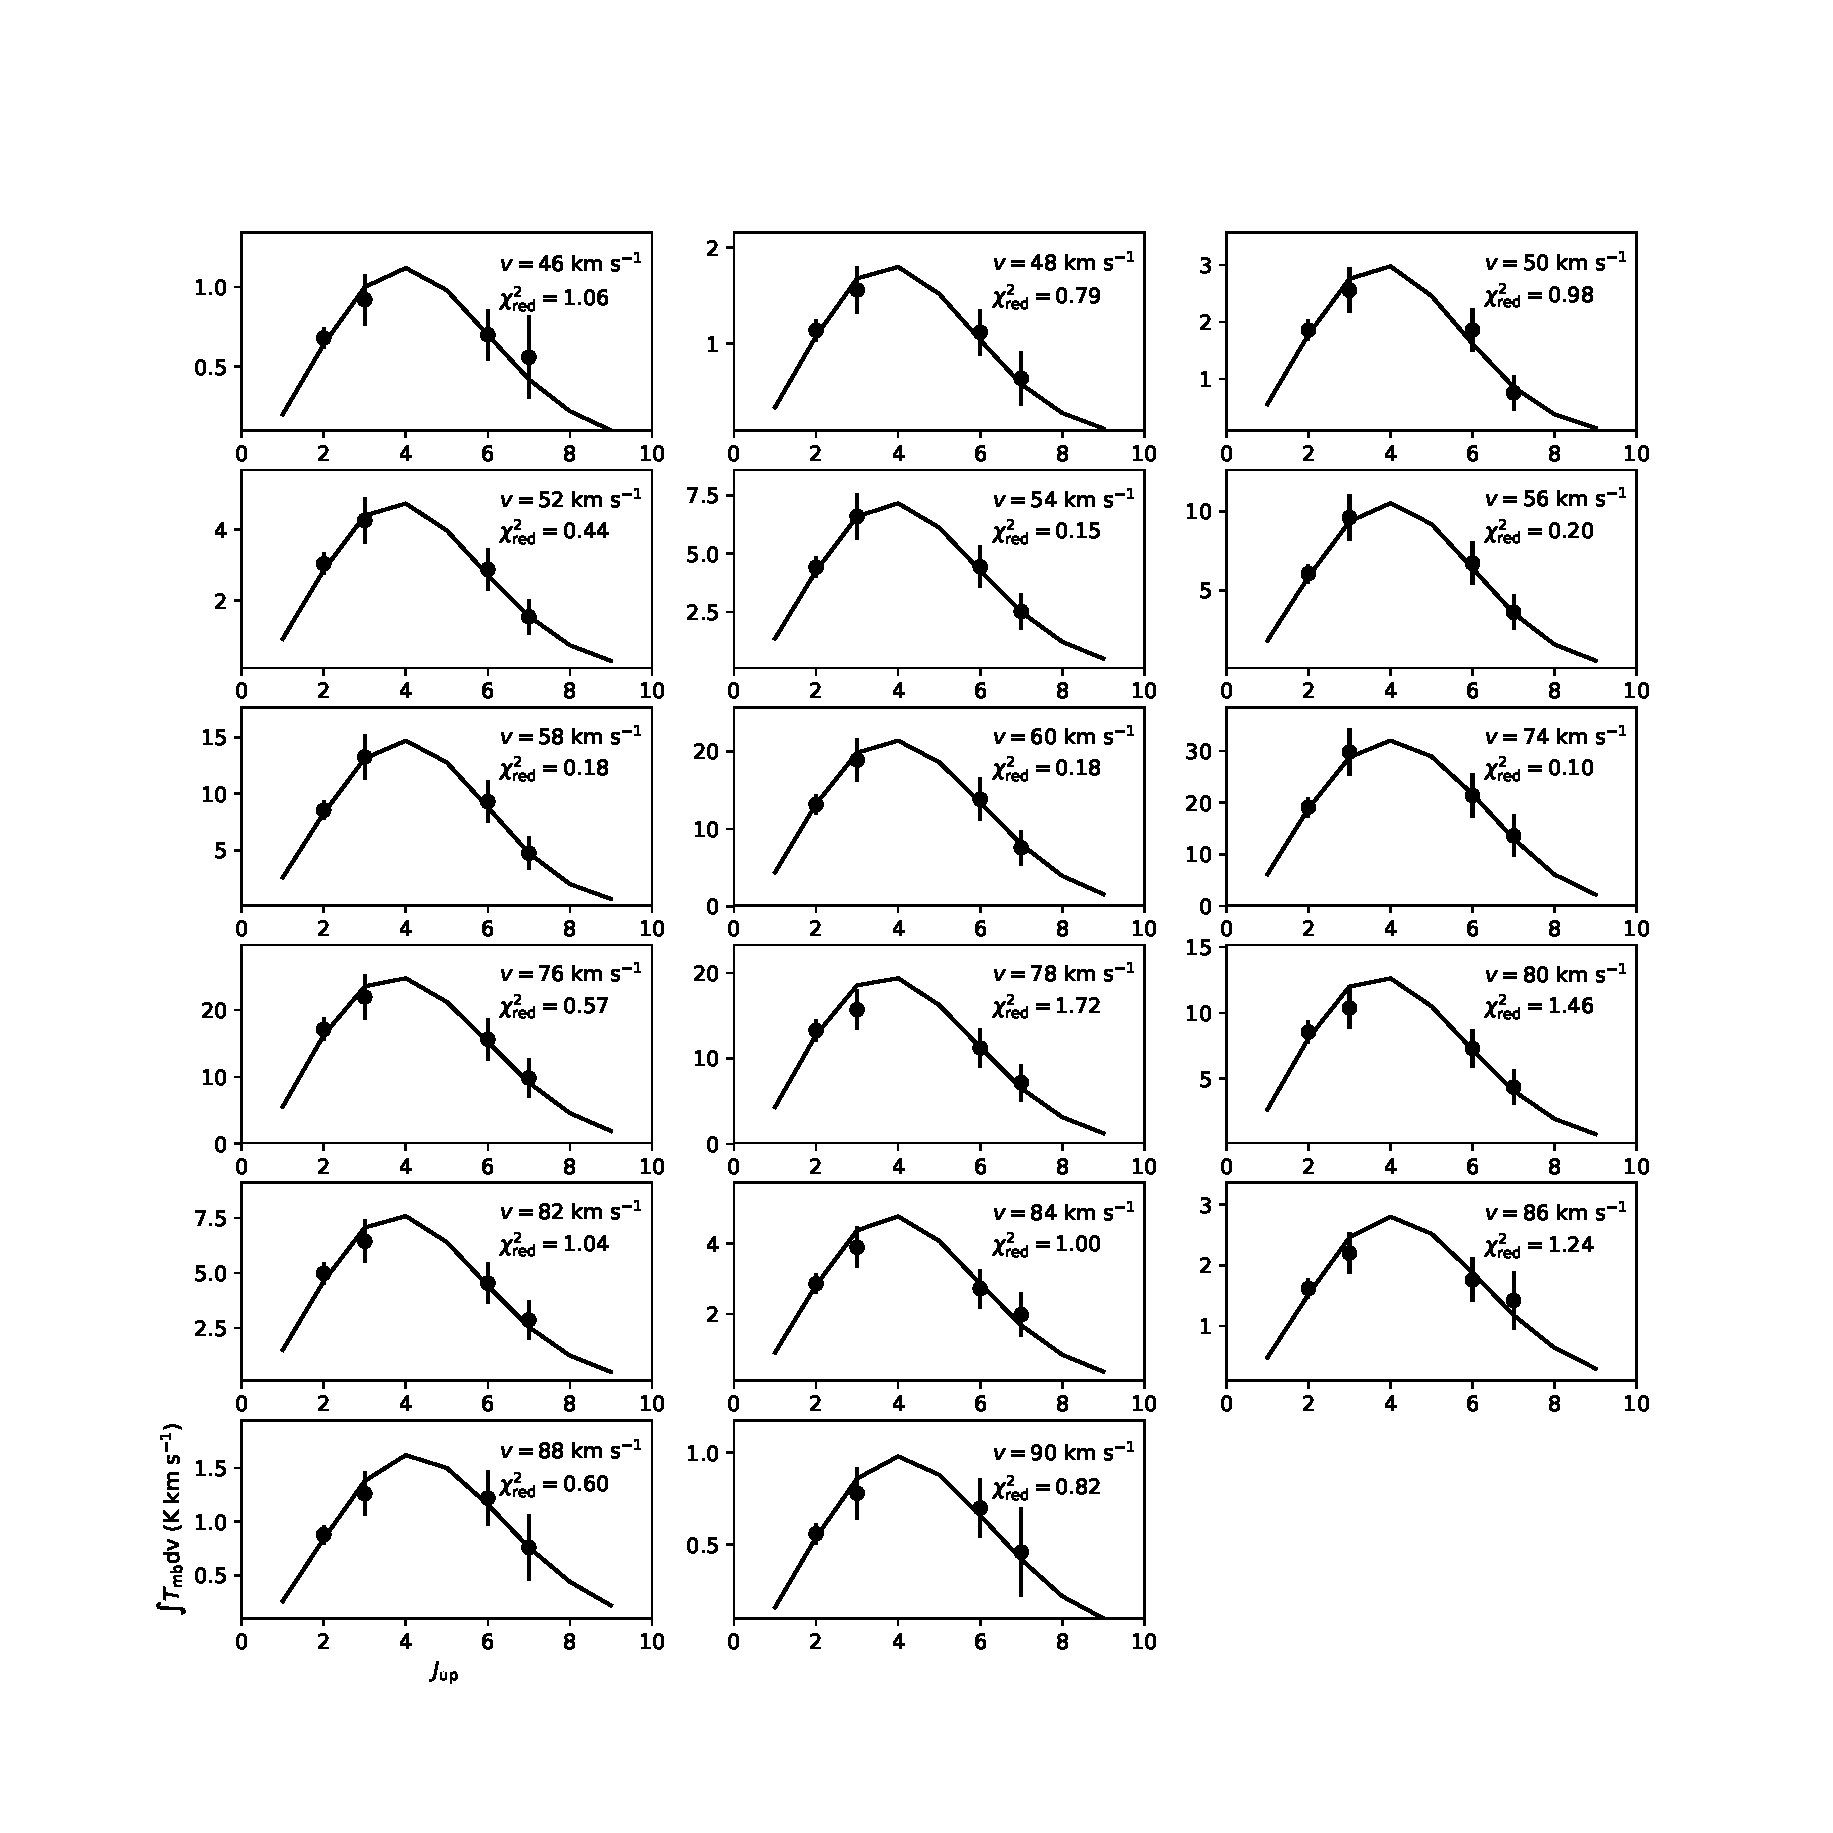
\includegraphics[scale=.60]{./fig/SED.eps}
\caption{Observed line fluxes compared with the LVG computations in each 2 km/s bin. The black solid circles show the observed data with error bars. The black solid lines refer to the best fits.  The $\chi^2_{\mathrm{red}}$ of the best fitting results and the outflow velocities are shown in each panel. \label{fig:figsed}}
\end{figure*}


\end{document}
